\section{Computational methods} \label{s:lit:computational}

\vspace{3mm}
% \noindent\rule{17cm}{0.2pt}
\fbox {
    \parbox{\linewidth}{
      \begin{itemize}
        \item Artificial Neural Networks
        \item Evolutionary Algorithms
        \item Networks
      \end{itemize}
    }
}
\vspace{3mm}

Machine Learning represents the collection of tools that are used in Artificial Intelligence development. According to \citet{Domingos_Pedro2015-xr}, there are five schools of thought in this area: the Symbolists, Analogizers, Bayesian, Connectionists, and Evolutionary. Symbolists are looking at drawing knowledge from logic symbols while the Analogizers are extrapolating information from mathematics and logic\cite{Domingos_Pedro2015-xr}. Connectionists and Evolutionary approaches take inspiration from biology, the former from the brain and the latter from Darwinian evolution. Bayesians are concerned with the uncertainty and are dealing with that probabilistic inference through Bayes's theorem\cite{Domingos_Pedro2015-xr}. As the readers will see in the following chapters most of the current work in bioinformatics uses Connectionists, Bayesian and sometimes Evolutionary approaches.

From an ML stance, learning can be of three types: supervised, semi-supervised and unsupervised learning. The first case is when the human labels the data, the corollary being that there is a need for careful processing as well as already having information about the data. This is the 'easiest' case as it comes with a wealth of information and the output is known to belong to the pre-defined set of labels. In supervised learning are the most recent progress in \acrfull{dl} was made but it is usually not a realistic scenario as labelling data is usually challenging and costly. 

The semi-supervised (or \acrfull{rl}) is when the model is not given labelled data to learn from, but a set of rules from where it needs to find the solution. This approach registered some successes through \acrfull{dqn} which achieved human skills at Atari games\cite{Mnih2015-cw} or AlphaGo Zero\cite{Silver2017-sw} which is the best Go player in the world. 

As the name suggests, the unsupervised learning is the case where there is no input from a human. These computational approaches are used when there is not enough data about the problem and what to expect, and patterns are hard to define. Clustering is the main algorithm used to find patterns in data which can then be validated with domain knowledge. 

The omics data are characterised by having a small number of samples with a relative large number of features, making it challenging to apply the supervised and semi-supervised learning algorithms. Especially on the disease stratification, unsupervised learning is more suitable as it is used to discover new patterns in the biological data.

This section covers the clustering techniques (\ref{s:lit:clustering}) to support the concepts in consensus subtyping (\ref{s:lit:rnaSeq}). Popular dimension reduction algorithms, covered in \cref{s:lit:dim_red}, are widely used in genomics where there is a high number of features. This is followed by EA (\ref{s:lit:ea_overview}) and Graph Theory (\ref{s:lit:graph_overview}) basics in order to support some of the work covered in the next section.

% Clustering analysis
\subsection{Clustering analysis} \label{s:lit:clustering}

Clustering algorithms have many variations, and these are best covered in a code sample \cite{Scikit-learn_undated-ax} from the Scikit-learn library \cite{Pedregosa2011-ts}. A selection of the methods that were successfully applied within this project is displayed in \cref{fig:lit:clustering_types}. The rows represent different types of datasets and the columns are the algorithms covered in this document: K-means as a general-purpose algorithm, and both Ward and Agglomerative as hierarchical clustering methods, with Agglomerative performing pairwise grouping. It is worth mentioning that a modified version of the Scikit-learn code was adapted to meet the project's needs, enabling the running of multiple clustering techniques with varied parameters for the TCGA dataset (\ref{}) and networks' outputs (\ref{}).

One of the most popular methods (and the simplest) is K-means clustering, which attempts to find patterns in the data by grouping data points by distance. There are variations of the algorithm where datasets are split into multiple batches to improve performance (see \textit{MiniBatch Kmeans} from \cref{fig:clustering_types}); or Fuzzy K-means that output the cluster membership of each data point. This means that apart from the cluster labelling, there is additional information about how close each point is to a cluster\footnote{For example, if there are 3 clusters, a data point might be 90\% in cluster 1, 6\% in cluster 2, and 4\% in cluster 3.}. From the below K-means pseudocode\footnote{Pseudocode is an accessible method to describe an algorithm.} (\cref{code:k-means}), it is worth emphasising the following:


\begin{figure}[!t]
  \centering
  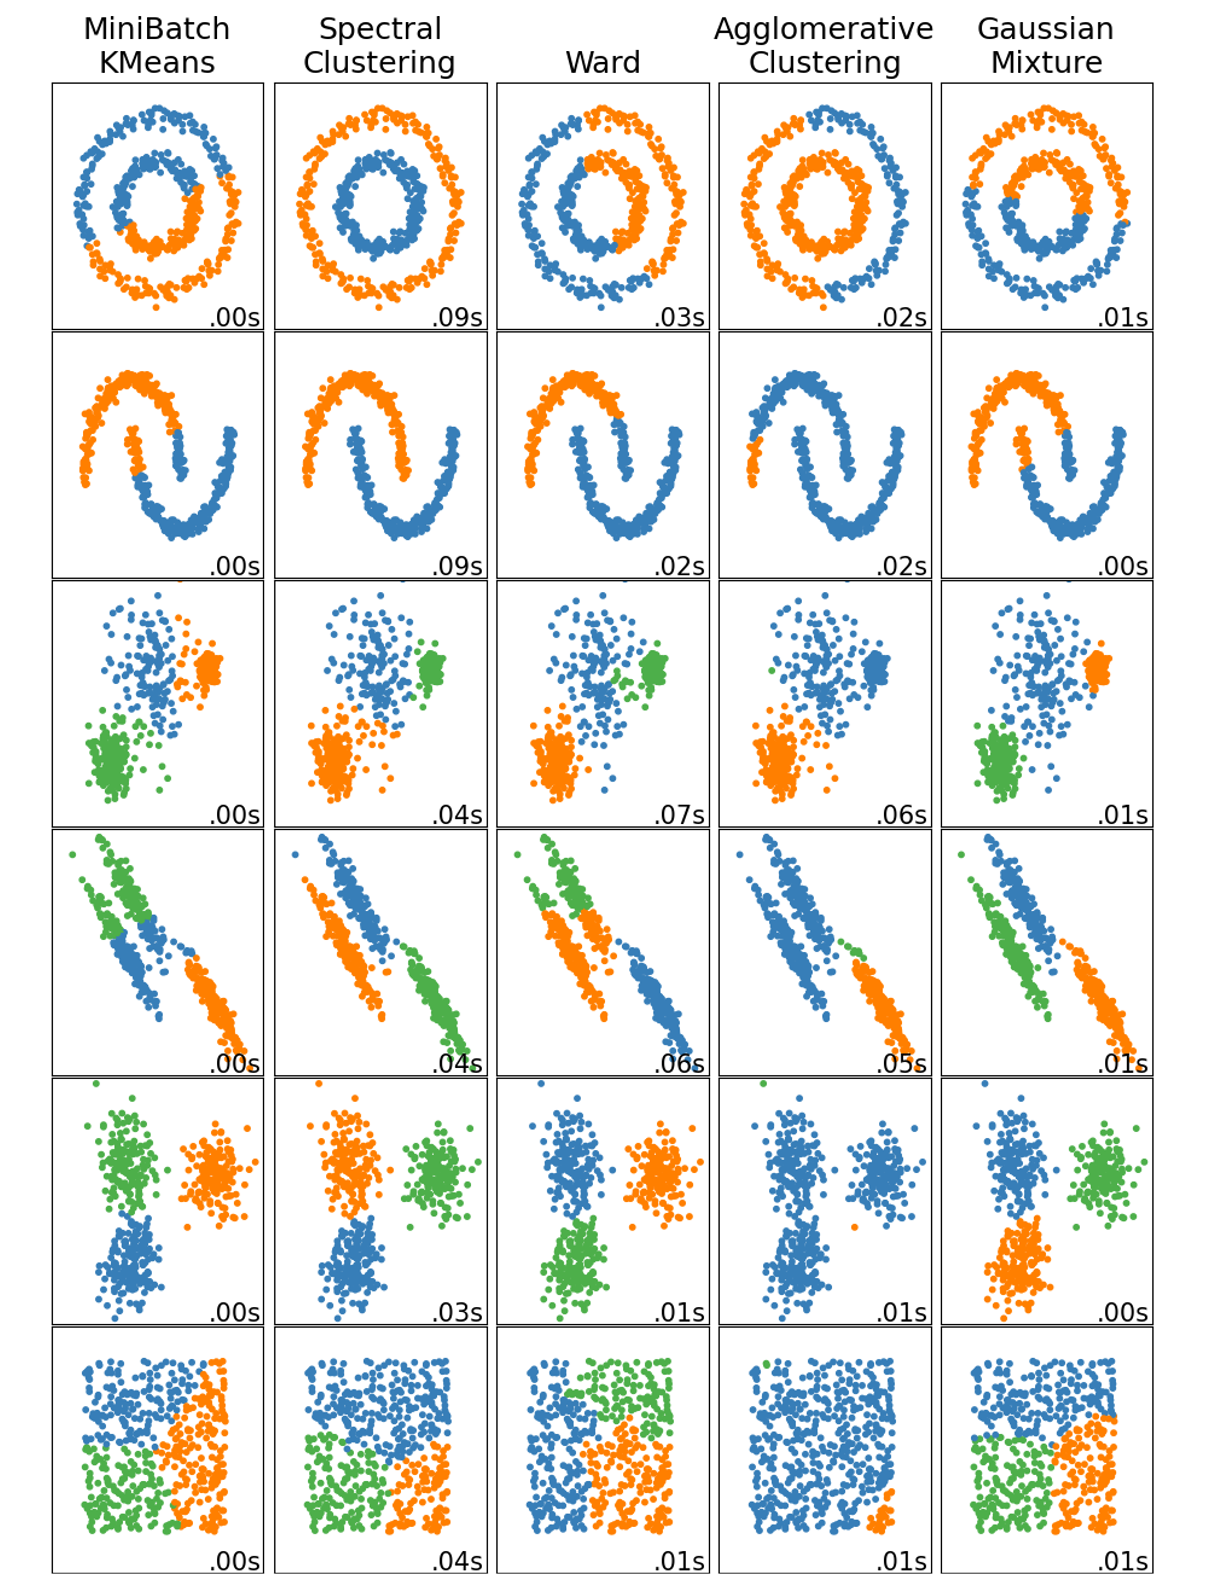
\includegraphics[width=0.8\textwidth,height=0.5\textheight,keepaspectratio]{Sections/Lit_review/Resources/clustering_scikit.png}
    \caption{How K-means (MiniBatch version), Spectral Clustering, Wards, Agglomerative Clustering, and Gaussian Mixture Models behave with different types of 2D datasets. Running times shown on the bottom right corner, all algorithms having comparable running times, with K-means being the fastest. Image adapted from \cite{Scikit-learn_undated-ax}}
    \label{fig:lit:clustering_types}
\end{figure}

\begin{itemize}
  \item The number of centroids (K) is defined by the user.
  \item The distance between two points can be of different types; the Euclidean is common, but for higher dimensions, cosine is more suitable.
  \item Even though the centroids are randomly initialised, new values are computed at each step by averaging the distance of the points in that cluster to the old centroid.
  \item The algorithm converges when the centroids do not significantly change.
\end{itemize}

\begin{lstlisting}[float=!hb, caption={K-means pseudocode}, label={code:k-means}]
  Initialise the centroids at random positions
  while not converged 
    For each data point
      Compute the distance to all the centroids
      The closest represents the cluster to which the data point belongs
    Update the centroids based on the mean distance of each cluster
\end{lstlisting} 

Agglomerative clustering is a type of hierarchical clustering that starts by considering each data point as its cluster and then computes higher up groups based on the given linkage method. These algorithms (pseudocode in \cref{code:agg_clustering}) build hierarchical trees and can be seen visually in dendrogram figures, which are useful in visualising the clustering evolution. Both K-means and Agglomerative Clustering can use different types of distances, but the latter does not require setting the number of centroids. However, the dendrogram  and the type of linkange method have to be chosen. This setting configures how the datapoint grouping is performed and the Scikit-learn supports the following\footnote{There is a nice visualisation for each of these hierarchical clustering in this \href{https://towardsdatascience.com/machine-learning-algorithms-part-12-hierarchical-agglomerative-clustering-example-in-python-1e18e0075019}{Medium post}}:
\begin{itemize}
  \item \textbf{Average} - Grouping is done by the average distance between cluster points.
  \item \textbf{Ward} - Merging clusters by the sum of squared distances. This linkage minimises the variance and is similar to K-means.
  \item \textbf{Single} - The distance between two groups is given by the two closest points. This considers merging clusters that have the closest points.
  \item \textbf{Complete} - The opposite to Single linkage, the distance between the two groups is given by the farthest points. This method looks at the outer layer points and may provide a more accurate grouping.
\end{itemize}


Gaussian Mixture Models (GMM) are probabilistic models that assume all data points are generated from a mixture of a finite number of Gaussian distributions with unknown parameters. GMMs accommodate asymmetric clusters compared to K-means which assumes clusters are similar in size. Another applied clustering algorithm in the project, Spectral Clustering, transforms the clustering problem into a graph-partitioning problem. It begins by constructing an affinity matrix based on the pairwise similarity of points. It then uses linear algebra to project the data into a latent space from which the clusters are identified using methods such as K-means.
~\\
\begin{lstlisting}[caption={Agglomerative hierarchical clustering pseudocode}, label={code:agg_clustering}]
  To each data point assign a cluster number
  while more than one cluster
    Group the closest datapoints together 
    Smaller clusters morph together into larger ones
\end{lstlisting} 

The clustering algorithms presented so far are used throughout the project, initially to establish a referential point independent of the methods used in other MIBC subtyping work \cite{Robertson2017-mg, Marzouka2018-ge, Kamoun2020-tj}. Then, the clustering models are used to stratify the output of the network approach. To measure the performance of these algorithms, the below metrics are used.



% Clustering metrics
\subsection{Clustering metrics} \label{s:lit:clustering_metrics}

One of the challenges in clustering is to measure the performance of grouping as there is no labelling or prior information on how the grouping should look like. This project uses the canonical metrics which are supported by Scikit-learn\cite{Pedregosa2011-ts,Scikit-learn_undated-ax}. These are:
\begin{itemize}
  \item \textbf{Silhouette Coefficient} - the higher the better. A higher Silhouette Coefficient score relates to a model with better-defined clusters. This is the preferred method in project for reasons highlighted in \ref{} and it has been used by the MIBC consensus \citet{Kamoun2020-tj} to asses the cluster separation.
  % It can use different distances and the score is calculated per sample as it follows:
  % \begin{itemize}
  %   \item The mean distance between a sample and all other points in a class.
  %   \item The mean distance between a sample and all other points in the next nearest cluster.
  %   \item The total score for the dataset is the mean of the above two points.
  % \end{itemize}
  \item \textbf{Calinski-Harabasz Index} - the higher the better. A higher Calinski-Harabasz score relates to a model with better-defined clusters.  The score is the ratio of the sum of between-clusters dispersion and of inter-cluster dispersion for all clusters (where dispersion is defined as the sum of distances squared).
  \item \textbf{Davies-Bouldin Index} - the lower the better. A lower Davies-Bouldin index relates to a model with better separation between the clusters. The index is the average ‘similarity’ between clusters, where the similarity is a measure that compares the distance between clusters with the size of the clusters themselves.
\end{itemize}


In addition to the above metrics, there is a popular heuristic procedure, the Elbow method, which aids in choosing the right number of clusters. In \cref{fig:elbow_method} the y-axis is represented by the distance of the points from their centroids, while the x-axis is the number of clusters. It can be seen that there is a point of inflexion when the number of clusters is set to five and that is considered to be the optimal number of clusters.

\begin{figure}[!htb]
  \centering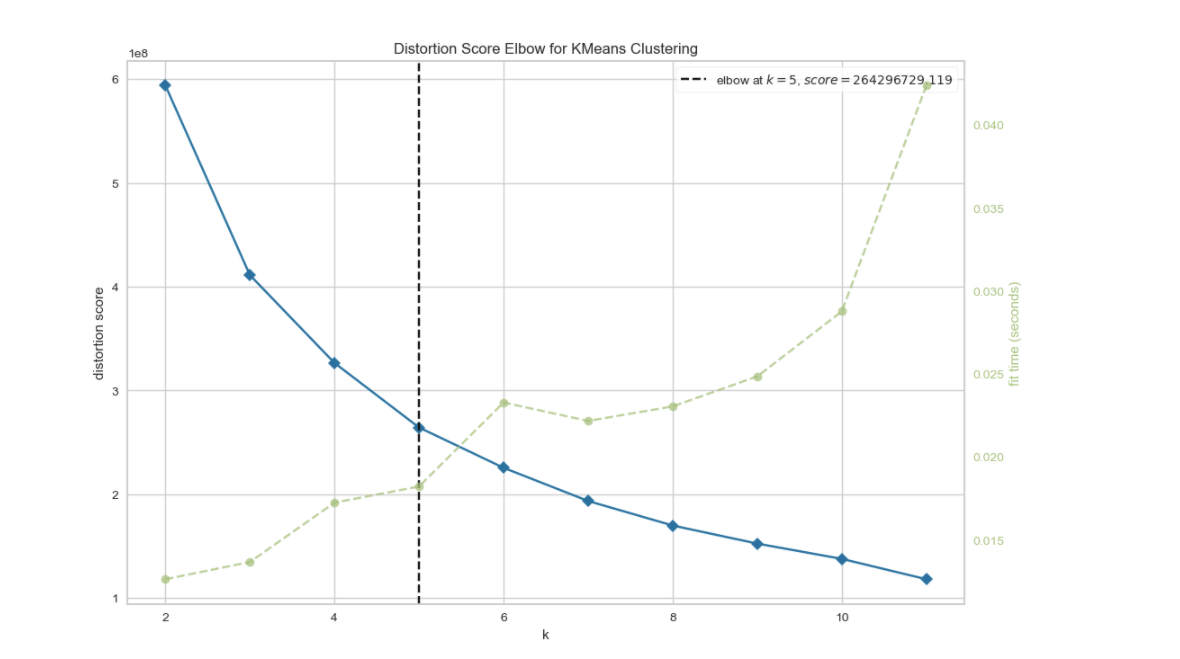
\includegraphics[width=0.8\textwidth,height=0.8\textheight,keepaspectratio]{Sections/Lit_review/Resources/elbow_method.png}
    \caption{Example of the elbow method, where 5 clusters are the optimal number of clusters. This has been applied to unpublished data of Benign Uropathies from Jack Birch Unit. The green line is the computational time. }
    \label{fig:elbow_method}
\end{figure}
\FloatBarrier

% Dimension reduction
\subsection{Dimension reduction} \label{s:lit:dim_red}

In contrast to many computationally- or physics-focused data analysis problems, biologically derived datasets are characterised by a high number of features (dimensions) and a small number of samples, making it necessary to use dimension reduction. \acrfull{pca} is the standard method which operates by projecting the higher dimension to the specified lower dimension. For example, a principal component of a genomic dataset might be linked to biological sex, as this influences many features of a biological system.

However, this does not align with non-linear patterns for which UMAP (Uniform Manifold Approximation and Projection) and t-SNE (t Distributed Stochastic Neighbour Embedding) are used. Both are stochastic and non-linear dimension reduction techniques widely used in bioinformatics. UMAP has been gaining popularity as it is more stable in representing both within and between cluster sample relatedness. While the method is good at reducing the data, its visualisation is misleading, as the proximity of points and clusters do not represent the 'closeness' of the data. When applying the two, one needs to use the clustering before, and then employ UMAP/t-SNE for visualisation.

Another dimension reduction technique is \acrfull{nmf} which operates on the same principles as PCA, which is by finding a matrix of a lower rank with the minimum information loss. This means that the features present in the data are preserved better when reduced to lower dimensions while the ones that do not contribute to the data resolution are discarded. Additionally, NMF conserves the non-linear aspects of the data and a Bayesian version of it is used in the \acrfull{tcga} classification by \citet{Robertson2017-mg}. NMF is also  used in the works of propagating (mutation) data into the networks by \citet{Yang2016-dm, Cai2008-fv} and is covered in \cref{s:lit:net_prop}.

PCA is extensively used in this project, initially to reduce the data in \ref{} (subtypes section), and subsequently as a proxy metric to gauge the amount of variance contained in a subset of genes. This approach has been particularly useful in the network chapters, where multiple graphs are generated, each outputting a different subset of genes for clustering the MIBC.

